% !TeX root = ../main_problemset.tex
\documentclass[../main_problemset.tex]{subfiles} % Inherits definitions from parent .tex file.

% Per-problem variable definitions
\newcommand{\problemName}{F. Balon Poligon}
\newcommand{\problemTL}{2 s}
\newcommand{\problemML}{64 MB}

\begin{document}

\begin{center}
    \section*{\problemName}
    \addcontentsline{toc}{section}{\problemName} % for pdf indexing
    
    \begin{tabular}{rl}
    Batasan waktu : & \problemTL \\
    Batasan memori : & \problemML
    \end{tabular}
\end{center}

\subsection*{Deskripsi}
\addcontentsline{toc}{subsection}{Deskripsi} % for pdf indexing

Pak Chanek memiliki sebuah balon 2D yang berbentuk poligon segi-M beraturan. Pada mulanya, balon tersebut kempes dan dapat dianggap sebagai sebuah titik. Awalnya, balon kempes tersebut terletak pada sebuah bidang Kartesius 2D, pada koordinat (0, 0).

Pada bidang Kartesius yang sama, terdapat N titik. Titik ke-i memiliki koordinat (X[i], Y[i]).

Apabila dipompa, balon akan terus mengembang dengan titik pusat (0, 0), sampai salah satu sisinya mengenai salah satu titik yang ada. Ukuran balon tersebut didefinisikan sebagai jarak antara titik pusat ke salah satu titik sudut balon.

Sebelum memompa, Pak Chanek dapat merotasi balon kempes tersebut sesuka hati.

Tentukan ukuran balon terbesar yang mungkin setelah dipompa!

\subsection*{Format Masukan}
\addcontentsline{toc}{subsection}{Format Masukan} % for pdf indexing

Baris pertama berisi sebuah bilangan bulat T yang menyatakan banyaknya kasus uji. Baris-baris berikutnya berisi T kasus uji, yang masing-masing diberikan dalam format berikut ini:

\begin{lcverbatim}
N M
X[1] Y[1]
X[2] Y[2]
.
.
X[N] Y[N]
\end{lcverbatim}

\subsection*{Format Keluaran}
\addcontentsline{toc}{subsection}{Format Keluaran} % for pdf indexing

Untuk setiap kasus uji, keluarkan sebuah baris berisi ukuran terbesar yang mungkin setelah dipompa. Jawaban akan dianggap benar apabila memiliki selisih absolut atau relatif dengan jawaban juri paling banyak sebesar $ 10^{-8} $.

\vspace{.4cm}

\begin{minipage}[t]{0.5\textwidth}
\subsection*{Contoh Masukan}
\addcontentsline{toc}{subsection}{Contoh Masukan} % for pdf indexing

\begin{lcverbatim}
3
1 3
2 4
2 3
2 2
2 4
4 4
-2 -2
2 -2
-2 2
2 2
\end{lcverbatim}
\end{minipage}
\begin{minipage}[t]{0.5\textwidth}
\subsection*{Contoh Keluaran}
\addcontentsline{toc}{subsection}{Contoh Keluaran} % for pdf indexing

\begin{lcverbatim}
8.944271909999
5.656854249492
4
\end{lcverbatim}
\end{minipage}

\textit{Perhatikan bahwa contoh kedua dan ketiga tidak termasuk dalam contoh masukan dan contoh keluaran dari soal versi mudah.}

\subsection*{Penjelasan}
\addcontentsline{toc}{subsection}{Penjelasan} % for pdf indexing

Berikut ini adalah ilustrasi untuk contoh pertama:

\begin{figure}[H]
	\centering
	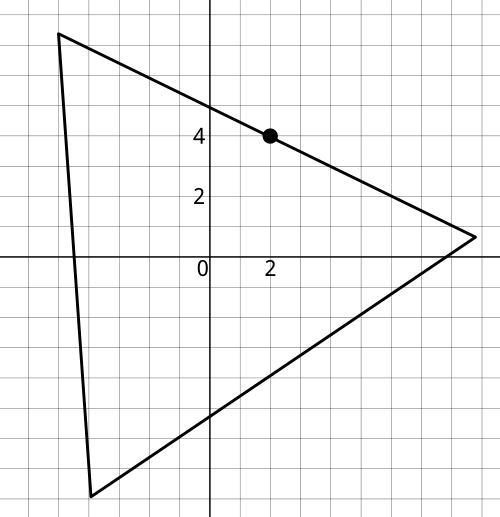
\includegraphics[width=225px]{balon/asset/1}
\end{figure}

Berikut ini adalah ilustrasi untuk contoh kedua:

\begin{figure}[H]
	\centering
	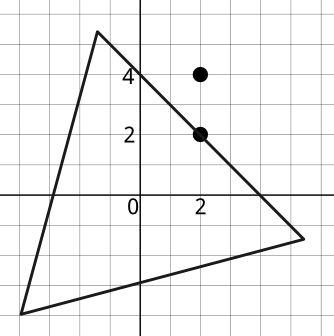
\includegraphics[width=150px]{balon/asset/2}
\end{figure}

Berikut ini adalah ilustrasi untuk contoh ketiga:

\begin{figure}[H]
	\centering
	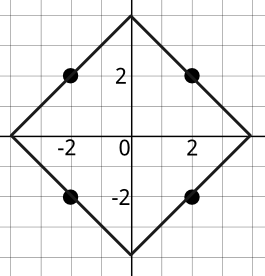
\includegraphics[width=120px]{balon/asset/3}
\end{figure}

\subsection*{Batasan}
\addcontentsline{toc}{subsection}{Batasan} % for pdf indexing

\begin{minipage}[t]{0.47\textwidth}

Batasan yang berlaku untuk versi mudah dan versi sulit:

\begin{itemize}
	\item 1 $ \leq $ T $ \leq $ 10
	\item 3 $ \leq $ M $ \leq $ 10
	\item -1.000.000 $ \le $ X[i], Y[i] $ \le $ 1.000.000
	\item (0, 0), (X[1], Y[1]), (X[2], Y[2]), ..., (X[N], Y[N]) dijamin merupakan titik-titik yang berbeda-beda
\end{itemize}
\end{minipage}
\begin{minipage}[t]{0.06\textwidth}
	\hfill
\end{minipage}
\begin{minipage}[t]{0.47\textwidth}
Batasan khusus versi mudah:
\begin{itemize}
	\item N = 1
\end{itemize}

\vspace{.2cm}

Batasan khusus versi sulit:
\begin{itemize}
	\item 1 $ \le $ N $ \le $ 100
\end{itemize}
\end{minipage}

\end{document}
